%LTeX: language=it
\chapter{2020-03-24}
\section{Sistemi di due particelle (reprise)}
\subsection{Energia, Impulso e Velocità di una particella nel sistema CM}
È nostro scopo ora calcolare le grandezze energia, impulso e velocità delle due
particelle nel sistema di riferimento del centro di massa (CM).

Nel sistema del centro di massa consideriamo come particella a riposo la
particella fittizia \textit{centro di massa} ed utilizziamo le equazioni
\ref{eq:sistema_riposo_altra} considerando appunto come particella di
riferimento la particella \textit{centro di massa}.

Rispetto alle equazioni \ref{eq:sistema_riposo_altra} avremo quindi che
\footnote{
	$\vec{P}$ è riferito alla particella CM
}:
\begin{equation}
	\begin{dcases}
		\qvec{P}_1 \rightarrow \qvec{P} = \qvec{P}_1 + \qvec{P}_2
		\\
		\qvec{P}_2 \rightarrow \qvec{P}_i \qquad \mrb{i = 1,2}
	\end{dcases}
\end{equation}

Quindi riscriviamo il set di equazioni \ref{eq:sistema_riposo_altra}:
\begin{equation}
	\begin{dcases}
		\eps_i^\ast = \frac{\qvec{P} \qvec{P}_i}{M}
		\\
		\abs{\vec{p}_i^{\,\ast}}^2
		= \frac{\mrb{\qvec{P} \qvec{P}_i}^2- M^2m_i^2}{M^2}
		\\
		\abs{\vec{\beta}_i}^{\ast2}
		= \frac{\mrb{\qvec{P}\qvec{P}_i}^2- M^2m_i^2}{\mrb{\qvec{P} \qvec{P}_i}^2}
	\end{dcases}
\end{equation}

Ricordiamoci che $\qvec{P}_i = \mcb{m_i,\, \vec{p}_i}$. Ci interessa ora sapere
l'espressione esplicita di $\qvec{P} \qvec{P}_i$, quindi:
\begin{subequations}
	\begin{equation}
		\qvec{P} \qvec{P}_i
		= \mrb{\qvec{P}_1 + \qvec{P}_2} \qvec{P}_i
		= \qvec{P}_1 \qvec{P}_i + \qvec{P}_2 \qvec{P}_i
	\end{equation}
	e poiché $i = 1, 2$, dunque:
	\begin{equation}
		\qvec{P} \qvec{P}_i
		= \qvec{P}_1 \qvec{P}_2 + \qvec{P}_i^2
		= \qvec{P}_1 \qvec{P}_2 + m_i^2
		= \frac{1}{2} \msb{M^2 - m_1^2 - m_2^2} + m_i^2
	\end{equation}
	Il primo termine della somma:
	\begin{equation}
		\qvec{P}_1 \qvec{P}_2
		= \frac{1}{2} \msb{\mrb{\qvec{P}_1 + \qvec{P}_2}^2 - \qvec{P_1}^2 -
			\qvec{P_2}^2}
		= \frac{1}{2} \msb{M^2 - m_1^2 - m_2^2}
	\end{equation}
	dove abbiamo sfruttato le relazioni fra la norma del quadrimpulso e la massa
	delle particelle. Sostituendo nell'equazione precedente si ottiene:
	\begin{equation}
		\boxed{
			\qvec{P} \qvec{P}_i
			= \frac{1}{2} \mrb{M^2 + m_i^2 - m_j^2} \qquad i,j
			= 1,2 \quad \text{e},
			\quad i\neq j
		}
	\end{equation}
\end{subequations}

Per le \textbf{energie} viste dal sistema del centro di massa:
\begin{equation}
	\boxed{\begin{dcases}
			\eps_1^\ast = \frac{M^2 + m_1^2 - m_2^2}{2M} \\
			\eps_2^\ast = \frac{M^2 + m_2^2 - m_1^2}{2M}
		\end{dcases}}
\end{equation}
vediamo che, nonostante nel sistema del centro di massa le due particelle
abbiano lo stesso impulso (in modulo), le energie sono diverse, causa le diverse
masse.

Osserviamo che la loro somma dovrebbe fornire la massa invariante $M$, infatti:
\begin{equation}
	\eps_1^\ast + \eps_2^*
	= \frac{M^2 + m_1^2 - m_2^2 + M^2 + m_2^2 - m_1^2}{2M}
	= \frac{2M^2}{2M}
	= M
\end{equation}

Per gli \textbf{impulsi} (\textit{trivettori}) visti dal sistema del centro di
massa:
\begin{equation}
	\abs{\vec{p}_{1}^{\ast}}^{2} = \frac{\mrb{M^2 + m_1^2 - m_2^2}^{2} - 4 M^2
		m_1^2}{4M^2}
\end{equation}
e analogamente per $\abs{\vec{p}_{2}^{\ast}}^{2}$, quindi svolgendo i calcoli:
\begin{equation}
	\boxed{
	\abs{\vec{p}^{\,\ast}}^2
	= \abs{\vec{p}_1^{\,\ast}}^2
	= \abs{\vec{p}_2^{\,\ast}}^2
	= \frac{\msb{M^2 - \mrb{m_1 + m_2}^2}\msb{M^2 - \mrb{m_1 - m_2}^2}}{4M^2}
	}
\end{equation}

\begin{example}[]
	Dimostrare che effettuando una trasformazione di Lorentz al CM si ottiene:
	\begin{equation}
		\vec{p}_1^{\,\ast} + \vec{p}_2^{\,\ast} = 0
	\end{equation}

	\begin{note}[]
		Ricordiamo che le quantità relative al SR del centro di massa sono indicate
		con il simbolo $\ast$.
	\end{note}

	Dimostriamo questa relazione utilizzando le trasformazioni di Lorentz nella
	forma vettoriale (equazione \ref{eq:lorentz_vettoriale}) e trasformiamo
	l'impulso come segue:
	\begin{equation}
		\vec{p}^{\,\ast} = \vec{p} - \vec{\beta}\gamma \msb{\frac{\gamma}{\gamma +
				1} \mrb{ -\vec{\beta} \cdot \vec{p}} + \eps} = \vec{p} + \vec{\beta}\gamma
		\msb{\frac{\gamma}{\gamma + 1} \mrb{\vec{\beta} \cdot \vec{p}} - \eps}
	\end{equation}

	Quindi scriviamo la trasformazione dell'impulso somma:
	\begin{equation}
		\vec{p}_1^{\,\ast} + \vec{p}_2^{\,\ast} = \vec{p}_1 + \vec{p}_2 +
		\vec{\beta}\gamma \msb{\frac{\gamma}{\gamma+1} \vec{\beta} \cdot
			\mrb{\vec{p}_1 + \vec{p}_2} - \mrb{\eps_1 + \eps_2}}
	\end{equation}
	Sfruttando il risultato dell'equazione \ref{eq:beta_CM}, sostituendo:
	\begin{equation}
		\vec{p}_1^{\,\ast} + \vec{p}_2^{\,\ast} = \vec{\beta} \mrb{\eps_1 +
			\eps_2} + \abs{\vec{\beta}}^2 \frac{\gamma^2}{\gamma + 1}
		\vec{\beta}\mrb{\eps_1 + \eps_2} - \gamma\vec{\beta}
	\end{equation}
	mettiamo in evidenza $\vec{\beta}\mrb{\eps_1 + \eps_2}$:
	\begin{equation}
		\vec{p}_1^{\,\ast} + \vec{p}_2^{\,\ast} = \vec{\beta}\mrb{\eps_1 +
			\eps_2} \msb{1 + \abs{\vec{\beta}}^2 \frac{\gamma^2}{\gamma + 1} -
			\gamma}
	\end{equation}
	Sfruttando la relazione:
	\begin{equation}
		\abs{\vec{\beta}}^2 = \frac{\gamma^2 - 1}{\gamma^2} = \frac{\mrb{\gamma -
				1} \mrb{\gamma + 1}}{\gamma^2}
	\end{equation}
	possiamo concludere quanto segue:
	\begin{align}
		\vec{p}_1^{\,\ast} + \vec{p}_2^{\,\ast}
		 & = \vec{\beta}\mrb{\eps_1 + \eps_2} \msb{1 + \frac{\mrb{\gamma - 1}
				\cancel{\mrb{\gamma + 1}}}{\cancel{\gamma^2}}
			\frac{\cancel{\gamma^2}}{\cancel{\gamma + 1}} - \gamma}
		\\\notag
		 & = \vec{\beta}\mrb{\eps_1 + \eps_2} \msb{\cancel{1} + \cancel{\gamma} -
			\cancel{1} - \cancel{\gamma}}
		\\\notag
		 & = 0
	\end{align}
	Quindi abbiamo dimostrato quanto era richiesto.
\end{example}

\begin{exercise}
	All'interno del nucleo, i nucleoni si muovono con energie cinetica
	dell'ordine di $\qty{20}{\MeV}$.
	Studiare gli effetti cinematici di questo movimento quando protoni di energia
	cinetica di $\qty{200}{\GeV}$ urtano i nucleoni nei casi in cui questi si
	muovano in direzione \textit{parallela} e \textit{antiparallela} ai protoni
	del fascio.
	Consideriamo per semplicità la massa dei nucleoni $\SI{1}{\frac{\GeV}{c^2}}$.
	\begin{enumerate}
		\item Calcolare la differenza di energia nel centro di massa nei casi
		      \textit{parallelo} e \textit{antiparallelo}.
		\item Quale energia dovrebbero avere i protoni incidenti per trovare la
		      stessa energia nel centro di massa se urtassero nucleoni a riposo?
	\end{enumerate}

	Il quadrimpulso totale nel caso \textit{parallelo}:
	\begin{equation}
		\qvec{P} = \Set{E_p + E_n, p_p + p_n, 0, 0}
	\end{equation}
	e nel caso \textit{antiparallelo}:
	\begin{equation}
		\qvec{P} = \Set{E_p + E_n, p_p - p_n, 0, 0}
	\end{equation}
	L'\textit{energia disponibile nel centro di massa} (invariante):
	\begin{align}
		\qvec{P}^2
		 & = E ^{\ast\, 2}
		\\\notag
		 & = \mrb{E_n + E_p}^{2} - \mrb{p_p \pm p_n}^{2}
		\\\notag
		 & = E_n^2 + E_p^2 + 2 E_p E_n - p_p^2 - p_n^2 \mp 2 p_p p_n
		\\\notag
		 & = \cancel{p_n^2} + m_n^2 + \cancel{p_p^2} + m_p^2 + 2 E_p E_n
		- \cancel{p_p^2} - \cancel{p_n^2} \mp 2 p_p p_n
		\\\notag
		 & = 2 m_n^2 + 2 E_p E_n \mp 2 \sqrt{\mrb{E_p^2 - m_n^2}\mrb{E_n^2 - m_n^2}}
	\end{align}
	dove nell'ultimo passaggio abbiamo considerato le masse dei nucleoni uguali
	in approssimazione $m_p = m_n$ e abbiamo sfruttato l'equazione
	$p_p p_n = \sqrt{\mrb{E_p^2 - m_n^2}\mrb{E_n^2 - m_n^2}}$.
	Indicando con $T_x$ l'energia cinetica:
	\begin{equation}
    T_p:
		\qquad
		E_p
		= T_p + m_n
		= \qty{200}{\GeV} + \qty{1}{\GeV}
		= \qty{201}{\GeV}
	\end{equation}
	\begin{equation}
    T_n:
		\qquad
		E_n
		= T_n + m_n
		= \qty{20}{\MeV} + \qty{1}{\GeV}
		= \qty{1.02}{\GeV}
	\end{equation}
	Quindi:
	\begin{equation}
		E ^{\ast\, 2} = 2 \mrb{1^2 + \numproduct[
				product-symbol = \ensuremath{\cdot}
			]{201 x 1.02} \mp 40.4} \unit{\GeV^2}
		= \begin{dcases}
			\qty{331.24}{\GeV^2}, \quad \textit{Parallelo}
			\\
			\qty{492.92}{\GeV^2}, \quad \textit{Antiparallelo}
		\end{dcases}
	\end{equation}
	allora:
	\begin{equation}
		E ^{\ast}
		= \begin{dcases}
			\qty{18.2}{\GeV}, \quad \textit{Parallelo}
			\\
			\qty{22.2}{\GeV}, \quad \textit{Antiparallelo}
		\end{dcases}
	\end{equation}

	Rispondendo alla seconda domanda:
	\begin{equation}
		\qvec{P}_n = \Set{E_n, 0, 0, 0}
	\end{equation}
	quindi:
	\begin{equation}
		E_n = \sqrt{\cancel{p_n^2} + m_n ^{2}} = m_n
	\end{equation}
	Dunque:
	\begin{equation}
		E_p \rightarrow E_p \mprime:
		\qquad
		E ^{\ast\, 2}
		= 2 m_n^2 + 2 E_p \mprime E_n \mp 2 \sqrt{\mrb{E_p^2 - m_n^2} \cancel{\mrb{m_n^2 - m_n^2}}}
		= 2 m_n^2 + 2 E_p \mprime E_n
	\end{equation}
	Allora scriviamo:
	\begin{equation}
		2 E_p \mprime E_n = E ^{\ast\, 2} - m_n^2
		\mthen
		E_p \mprime
		= \frac{1}{2 m_n} \msb{E ^{\ast`, 2} - 2 m_n^2}
		= \frac{E ^{\ast\, 2} - 2}{2}
	\end{equation}
	Infine:
	\begin{equation}
		E _{p} \mprime
		= \begin{dcases}
			???, \quad \textit{Parallelo}
			\\
			\qty{245}{\GeV}, \quad \textit{Antiparallelo}
		\end{dcases}
	\end{equation}
\end{exercise}

\section{Decadimento in due corpi}
Trattiamo ora il caso di una particella $\boldsymbol{A}$ che decade in due
particelle $\boldsymbol{B}$ e $\boldsymbol{C}$ (figura
\ref{fig:decadimento_due_corpi}) nel sistema del centro di massa (CM).
L'energia disponibile nel centro di massa è proprio l'energia a riposo della
particella iniziale $\boldsymbol{A}$ ed è la quantità  $E^\ast = M$.
Dopo il decadimento, chiaramente: $M \rightarrow m_1 + m_2$.

\begin{figure}[ht!]
	\centering
	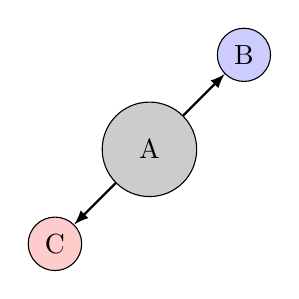
\begin{tikzpicture}[scale=0.8]
		\node[circle, draw, fill=black!20, minimum size = 1.2cm] (A) at (0,0) {A};
		\node[circle, draw, fill=blue!20, minimum size = 0.4cm] (B) at (1.5,1.5) {B};
		\node[circle, draw, fill=red!20, minimum size = 0.4cm] (C) at (-1.5,-1.5) {C};

		\draw[-latex, thick] (A)--(B);
		\draw[-latex, thick] (A)--(C);
	\end{tikzpicture}
	\caption{Schema del decadimento in due corpi nel sistema del centro di massa}
	\label{fig:decadimento_due_corpi}
\end{figure}

Per il sistema vale:
\begin{equation}
	\begin{dcases}
		\vec{p}_1 + \vec{p}_2 = 0
		\\
		\eps_1^\ast + \eps_2^\ast = E ^{\ast} = M
	\end{dcases}
\end{equation}
dove:
\begin{equation}
	\eps_1^\ast = \frac{M^2 + \mrb{m_1 + m_2}^2}{2M};
	\qquad
	\eps_2^\ast = \frac{M^2 + \mrb{m_1^2 - m_2^2}}{2M}
\end{equation}
\begin{equation}
	\abs{\vec{p}^{\,\ast}}^2
	= \abs{\vec{p}_{1}^{\ast}}^{2}
	= \abs{\vec{p}_{2}^{\ast}}^{2}
	= \frac{\msb{M^2 - \mrb{m_1 + m_2}^2} \msb{M^2 -
			\mrb{m_1 - m_2}^2}}{4M^2}
	\label{eq:modulo_quadro_impulso}
\end{equation}

\begin{note}[]
	In questo schema di decadimento abbiamo considerato una distribuzione
	\textit{isotropa} degli impulsi risultati dal decadimento. Questa condizione
	d'isotropia, tuttavia, può essere fortemente alterata dalla dinamica interna
	del sistema, che noi in questo caso stiamo trascurando. Questo vuol dire che
	non è detto che la direzione degli impulsi risultanti sia soggetta a una
	condizione d'isotropia.
\end{note}

\begin{example}[]
	Consideriamo il caso di un decadimento di un \textit{pione positivo} $\pi^+$
	in un \textit{muone positivo} $\mu^+$ e in un \textit{neutrino muonico}
	$\nu_\mu$:
	\begin{equation}
		\pi^+ \longrightarrow \mu^+ + \nu_\mu
	\end{equation}
	Le masse delle particelle:
	\begin{align}
		m_\pi = \qty{140}{\MeV\per c^2};
		\qquad
		m_\mu = \qty{106}{\MeV\per c^2};
		\qquad
		m_\nu = \qty{0}{\MeV\per c^2}
	\end{align}
	Sfruttando i risultati che abbiamo ricavato fino a ora, nel sistema del
	centro di massa abbiamo:
	\begin{subequations}
		\begin{equation}
			\abs{\vec{p}_\mu^{\,\ast}}^2 = \abs{\vec{p}_\nu^{\,\ast}}^2
			= \frac{
				\msb{m_\pi^2 - \mrb{m_\mu^2 + \cancel{m _{\nu}^{2}}}}
				\mrb{m_\pi^2 - \mrb{m_\mu^2 - \cancel{m _{\nu}^{2}}}}
			}{4m_\pi^2}
			= \frac{\mrb{m_\pi^2 - m_\mu^2}\mrb{m_\pi^2 - m_\mu^2}}{4m_\pi^2}
			= \frac{\mrb{m _{\pi}^{2} - m _{\mu}^{2}}^{2}}{4 m _{\pi}^{2}}
		\end{equation}
		\begin{equation}
			\Rightarrow \abs{\vec{p}_\mu^{\,\ast}}
			= \abs{\vec{p}_\nu^{\,\ast}}
			= \frac{m_\pi^2 - m_\mu^2}{2m_\mu}
			= \frac{140^2-106^2}{\numproduct[
					product-symbol = \ensuremath{\cdot}
				]{2 x 140}}\si{\MeV\per c}
			\simeq \qty{30}{\MeV\per c}
		\end{equation}
	\end{subequations}

	Per le energie abbiamo:
	\begin{equation}
		\eps_\mu = \sqrt{\abs{\vec{p}_\mu^{\,\ast}}^2 + m_\mu^2}
		\simeq \qty{110}{\MeV};
		\qquad
		\eps_\nu = \sqrt{\abs{\vec{p}_\nu^{\,\ast}}^2 + m_\nu^2}
		\simeq \qty{30}{\MeV}
	\end{equation}
\end{example}

\begin{example}[]
  Consideriamo il caso del decadimento della particella $\Lambda$\footnote{
    $\Lambda$ è una particella neutra; In tutte le reazioni valgono:
    \begin{itemize}
      \item \textit{principio di conservazione della carica}
      \item \textit{principio di conservazione del numero leptonico}
      \item \textit{principio di conservazione del numero barionico}
    \end{itemize}
  }:
	\begin{equation}
		\Lambda \rightarrow p + \pi ^{-}
	\end{equation}
  Date le masse:
  \begin{equation}
    m _{\Lambda} = \qty{1116}{\MeV \per c^2};
    \qquad
    m_p = \qty{938}{\MeV \per c^2};
    \qquad
    m _{\pi^-} = \qty{140}{\MeV \per c^2}
  \end{equation}
	Abbiamo, nel sistema di riposo della particella $\Lambda$ che decade, che
  coincide con il sistema del centro di massa:
	\begin{equation}
		\abs{\vec{p}_{p}^{\,\ast}}^{2}
		= \abs{\vec{p}_{\pi^-}^{\,\ast}}^{2}
		= \frac{
			\msb{m _{\Lambda} ^{2} - \mrb{m _{p} + m _{\pi}}^{2}}
			\msb{m _{\Lambda} ^{2} - \mrb{m _{p} - m _{\pi}}^{2}}
		}{4 M _{\Lambda}^{2}}
    \simeq \qty{101}{\MeV \per c}
	\end{equation}
\end{example}
